\documentclass[11pt]{article}

% -----------------------------------------------------------------------------
% Publisher-neutral manuscript shell. Replace the document class only after the
% target journal has been selected; section files are deliberately modular.
% -----------------------------------------------------------------------------
\usepackage[margin=1in]{geometry}
\usepackage{graphicx}
\usepackage{booktabs}
\usepackage{multirow}
\usepackage{tabularx}
\usepackage{array}
\usepackage{amsmath,amssymb}
\usepackage{microtype}
\usepackage{enumitem}
\usepackage{hyperref}
\usepackage{cleveref}
\usepackage{natbib}
\usepackage{xcolor}

\hypersetup{
  colorlinks=true,
  linkcolor=blue,
  citecolor=blue,
  urlcolor=blue
}

\newcommand{\pcste}{PC-STE}
\newcommand{\fulls}{Full-S1}
\newcommand{\kone}{K1}
\newcommand{\qeight}{Q8(K1)}
\newcommand{\macrofour}{Macro-4}

\title{\textbf{Lightweight PC-STE: Performance-Preserving Compression of a Shared Multi-Dataset State-Space Encoder for Rotating-Machinery Fault Diagnosis}}

\author{
Mohammad Abdalaziz$^{1}$ \and
Erick Giovani Sperandio Nascimento$^{1}$ \and
Marco Aur\'elio da Silva Cruz$^{1}$
}

\date{}

\begin{document}

\maketitle

\begin{center}
$^{1}$\textit{University of Surrey, Guildford, United Kingdom.}\\
\textit{Corresponding author to be designated before submission.}
\end{center}

\begin{abstract}
Reusable vibration encoders can reduce the need to develop a separate diagnostic model for every machinery dataset, but their computational cost can hinder deployment. This work investigates whether a shared multi-dataset selective-state-space encoder can be compressed without an unacceptable loss of diagnostic performance. The reference model, Full-S1, is a self-supervised PC-STE encoder with four bidirectional Mamba layers and dataset-specific heads for CWRU, JNU, HIT, and MaFaulDa. A lightweight student, K1, is structurally derived by retaining the four temporal stages while removing the reverse selective-scan path. K1 is distilled from a same-fold ensemble of three independently seeded Full-S1 teachers. Evaluation uses three global folds and three seeds, yielding nine matched teacher--student cells, with a prespecified $-0.02$ Macro-F1 non-inferiority margin. K1 increases equal-domain Macro-F1 from $0.934644\pm0.023258$ to $0.955334\pm0.018393$ and satisfies the predefined non-inferiority criterion (exact one-sided sign-flip $p=0.001953125$). Structurally, K1 reduces encoder parameters by $42.24\%$, serialized FP32 size by $42.14\%$, and computation by $45.38\%$. Corrected deployment measurements show $1.874\times$ CPU and $1.633\times$ GPU end-to-end batch-1 speed-ups and approximately $2.0\times$ GPU batch-32 throughput. A secondary post-training Q8 extension preserves the simulated-Q8 predictive result while reducing stored model size by a further $71.12\%$ relative to K1 FP32. The results show that directionality-specific state-space compression combined with ensemble distillation can substantially reduce inference cost while retaining the diagnostic performance of a shared vibration representation.
\end{abstract}

\noindent\textbf{Keywords:} predictive maintenance; rotating machinery; fault diagnosis; state-space models; Mamba; knowledge distillation; model compression; quantization

\section{Introduction}
\label{sec:introduction}

Rotating machinery is central to manufacturing, transportation, energy, and other asset-intensive industrial systems, where unexpected failures can interrupt production, increase maintenance expenditure, and compromise operational safety. Predictive and condition-based maintenance seek to reduce these risks by using condition-monitoring information to support timely diagnostic and maintenance decisions \citep{Jardine2006CBM,Nunes2023Challenges}. Among the available condition-monitoring modalities, vibration signals remain particularly important because bearing, rotor, and other mechanical defects modify the temporal and spectral structure of the measured response. The increasing availability of industrial sensing and computing has consequently driven a transition from manually engineered diagnostic features toward data-driven and deep-learning methods for machine health monitoring \citep{Zhao2019DLHealth,Souza2021RotatingDL,Nascimento2022T4PdM}.

Deep neural networks can learn discriminative fault representations directly from measured signals, but many diagnostic models remain closely tied to a particular dataset, machine configuration, or label space. This limits reuse when fault classes, sampling conditions, and acquisition systems change. Recent research has therefore moved beyond purely task-specific classifiers toward reusable pretrained representations. FaultFormer demonstrated self-supervised masked pretraining for bearing vibration signals and subsequent adaptation to low-data and cross-dataset settings \citep{Zhou2024FaultFormer}; BearingFM proposed a foundation-style bearing model using domain knowledge and contrastive learning \citep{Lai2024BearingFM}; and RmGPT introduced a unified pretrained framework for rotating-machinery diagnosis and prognosis \citep{Wang2025RmGPT}. More recently, VibFM scaled masked spectrogram modelling to 16 open vibration datasets and evaluated transfer to held-out bearing datasets \citep{Mannone2026VibFM}. These developments indicate a clear shift toward representations that can support multiple diagnostic tasks rather than a separate network for every individual dataset.

At the same time, sequence modelling for machinery diagnosis has begun to adopt state-space architectures. Mamba introduced selective state-space modelling as an alternative to attention-based sequence processing, with input-dependent state updates and linear sequence scaling \citep{Gu2023Mamba}. In rotating-machinery applications, MD-BiMamba employed bidirectional Mamba processing for inter-shaft bearing diagnosis \citep{Wang2025MDBiMamba}, while VibrMamba combined bidirectional state-space processing with lightweight projection layers and evaluated six classification tasks across four public machinery datasets \citep{Yi2025VibrMamba}. These studies show that Mamba-based and lightweight Mamba-based fault diagnosis are already established research directions. Consequently, the relevant deployment question is no longer whether a compact Mamba classifier can be designed, but whether an already trained reusable state-space representation can be compressed in a controlled manner without introducing an unacceptable loss of diagnostic capability.

This question is important because reusable encoders can still impose substantial computational and storage costs at inference time. In industrial deployment, model quality must be balanced against memory footprint, arithmetic complexity, latency, throughput, and the capabilities of the target hardware. Knowledge distillation and structural compression have therefore received increasing attention in bearing diagnosis. DTCP-MAKD combines decreasing-threshold channel pruning with multi-assistant knowledge distillation to bridge the capacity gap between teacher and student models \citep{Zhong2024DTCPMAKD}; BFD-KD uses multiple teachers with dynamic weighting and intermediate-feature fusion for lightweight rolling-bearing diagnosis \citep{Sun2026BFDKD}; and BearingPGA-Net combines decoupled knowledge distillation, customized quantization, and FPGA acceleration for deployable bearing diagnosis \citep{Liao2024BearingPGANet}. These works demonstrate that structural reduction, multi-teacher supervision, quantization, and hardware-oriented deployment are not individually new. However, they primarily compress task-specific diagnostic networks or directly design lightweight architectures rather than examining the compression of a shared multi-dataset selective-state-space encoder.

The distinction is relevant for the present study. The full Physical-Coordinate Spectro-Temporal Encoder (PC-STE) uses one shared encoder across CWRU, JNU, HIT, and MaFaulDa, with dataset-specific classification heads. Its Full-S1 configuration is initialized through masked spectrogram reconstruction and employs four bidirectional temporal Mamba blocks together with physical time--frequency coordinates and cross-band mixing. The purpose of the present work is not to re-establish self-supervised pretraining, Mamba-based fault diagnosis, or multi-teacher knowledge distillation as new concepts. Instead, it addresses a narrower deployment problem: \emph{can a shared multi-dataset bidirectional state-space encoder be structurally compressed while retaining its diagnostic performance and delivering measurable computational benefits?}

To investigate this question, the bidirectional Full-S1 encoder is structurally reduced to K1, a four-layer forward-only student that removes the reverse temporal scan while preserving the remaining encoder hierarchy and the shared multi-dataset role. K1 is then trained by knowledge distillation from an ensemble of three independently seeded Full-S1 teachers from the same global fold. This teacher construction differs from heterogeneous multi-teacher or pruning-derived teacher-assistant schemes: all teachers share the same architecture, fold, task definition, and training protocol, with their diversity arising primarily from stochastic optimization. The resulting student is evaluated as a compression of the existing encoder rather than as an unrelated small model designed from scratch.

A central methodological feature of the study is that compression is treated as a \emph{performance-retention} problem. The final Full-S1--K1 comparison uses three global folds and three matched random seeds, yielding nine paired experimental cells. Before final TEST evaluation, a Macro-F1 non-inferiority margin of $-0.02$ was fixed to define the largest acceptable loss in the equal-domain Macro-4 endpoint. This design permits the efficiency gain to be assessed against an explicit retention criterion rather than through a single accuracy comparison or an informal statement of ``minimal degradation.'' Computational evaluation is performed separately using fixed validation inputs and a common hardware environment, with parameter count, serialized size, FLOPs, corrected CPU/GPU latency, throughput, and GPU memory reported under controlled conditions. A post-training Q8 stage is additionally examined as a secondary deployment extension and is kept distinct from the primary Full-S1--K1 confirmatory study.

The final results show that structural compression does not require a loss of aggregate diagnostic performance in this setting. Across the nine matched cells, Macro-4 Macro-F1 increases from $0.934644\pm0.023258$ for Full-S1 to $0.955334\pm0.018393$ for K1, corresponding to a paired change of $+0.020691\pm0.013509$, with K1 higher in eight of the nine cells. The predefined non-inferiority criterion is satisfied by the exact paired sign-flip test ($p=0.001953125$). At the same time, K1 reduces encoder parameters by $42.24\%$, serialized FP32 model size by $42.14\%$, and equal-domain computational cost by $45.38\%$. Under the corrected inference benchmark, K1 provides a $1.874\times$ end-to-end CPU batch-1 speed-up, a $1.633\times$ end-to-end GPU batch-1 speed-up, and approximately $2.0\times$ GPU batch-32 throughput. The secondary Q8 representation retains essentially the same aggregate Macro-F1 while reducing stored model size by a further $71.12\%$ relative to K1 FP32; because the preserved implementation has no true INT8 CUDA path, Q8 is interpreted primarily as a storage and CPU-deployment extension rather than a GPU acceleration result. The study therefore focuses on multi-dataset performance retention and deployment efficiency, not on claims of unseen-machine generalization.

\paragraph{Contributions.}
The main contributions of this study are summarized as follows:
\begin{enumerate}[leftmargin=*,label=(\roman*)]
    \item \textbf{Directionality-specific structural compression of a shared PC-STE encoder.}
    The bidirectional Full-S1 selective-state-space encoder is structurally reduced to a forward-only four-layer K1 student while retaining one shared encoder across CWRU, JNU, HIT, and MaFaulDa with dataset-specific classification heads.

    \item \textbf{Ensemble knowledge distillation for the compressed encoder.}
    K1 is distilled from same-fold, independently seeded Full-S1 teachers, combining classification distillation with relational supervision while preserving a single compact inference model.

    \item \textbf{Matched performance-retention evaluation.}
    The teacher--student comparison uses three global folds and three random seeds, producing nine matched cells, together with a prespecified $-0.02$ Macro-F1 non-inferiority margin to assess whether compression introduces an unacceptable diagnostic-performance loss.

    \item \textbf{Controlled predictive--efficiency characterization with a secondary Q8 extension.}
    The study reports model size, parameter count, FLOPs, corrected CPU/GPU latency, throughput, and memory under one controlled benchmark environment, and additionally evaluates post-training Q8 quantization as a secondary deployment extension.
\end{enumerate}

The remainder of this paper is organized as follows. Section~\ref{sec:literature} reviews self-supervised and foundation-style vibration models, Mamba-based machinery diagnosis, lightweight fault-diagnosis approaches, and deployment-oriented compression. Section~\ref{sec:methodology} presents the datasets, PC-STE representation, Full-S1 reference model, K1 structural compression, ensemble distillation, Q8 extension, and evaluation protocol. Section~\ref{sec:results} reports predictive performance, non-inferiority analysis, computational efficiency, and Q8 results. Finally, Section~\ref{sec:conclusion} summarizes the main findings, limitations, and future work.

\section{Review of Literature}
\label{sec:literature}

Research on data-driven rotating-machinery diagnosis has progressed from task-specific convolutional and recurrent models toward reusable representations, state-space sequence models, and deployment-oriented compression. These directions are related but address different problems. The present work is positioned at their intersection: the objective is not to introduce Mamba, self-supervised vibration learning, or knowledge distillation independently, but to study controlled compression of a shared multi-dataset state-space encoder and to evaluate the resulting performance--efficiency trade-off.

\subsection{Self-Supervised and Foundation Models for Vibration Diagnosis}
\label{subsec:foundation}

Deep-learning methods have become established tools for learning diagnostic representations directly from vibration measurements, reducing dependence on manually designed features \citep{Zhao2019DLHealth,Souza2021RotatingDL}. Nevertheless, conventional supervised models are commonly optimized for a fixed dataset and label space. Reusing them under new machines, sensing arrangements, or class taxonomies can require substantial retraining. This limitation has motivated self-supervised and foundation-style approaches that learn more transferable representations before downstream supervision.

FaultFormer is an early example of this direction in bearing diagnosis, using masked self-supervised pretraining and subsequent adaptation to downstream classification \citep{Zhou2024FaultFormer}. BearingFM further develops the idea of a reusable bearing representation through domain-informed augmentation and contrastive learning \citep{Lai2024BearingFM}. RmGPT broadens the scope by proposing a unified pretrained framework for diagnosis and prognosis in rotating machinery \citep{Wang2025RmGPT}. More recently, VibFM applies masked spectrogram modelling across 16 open vibration datasets and evaluates transfer to held-out datasets \citep{Mannone2026VibFM}. Collectively, these studies demonstrate that reusable vibration representations and multi-dataset pretraining are now active, established research directions.

This progression changes the deployment problem. When a representation is intended to support several downstream datasets or tasks, deployment is no longer only a matter of designing a small classifier. A reusable encoder can itself become the computational bottleneck. The question addressed in this paper is therefore downstream of foundation-style representation learning: once a shared representation has been learned, can its state-space backbone be structurally reduced while preserving the diagnostic behaviour that made the shared model useful in the first place?

\subsection{State-Space and Mamba Models for Machinery Diagnosis}
\label{subsec:mamba}

Transformers have demonstrated strong sequence-modelling capability in predictive-maintenance applications, including rotating-machinery diagnosis \citep{Nascimento2022T4PdM}. Their attention mechanism, however, can become expensive as sequence length increases. Selective state-space models provide a different approach. Mamba introduces input-dependent state updates while retaining linear scaling with sequence length \citep{Gu2023Mamba}. This combination has encouraged rapid adoption of Mamba-style architectures in time-series and machinery-diagnostic applications.

In rotating machinery, MD-BiMamba uses bidirectional Mamba processing together with modal decomposition and feature fusion for aero-engine inter-shaft bearing diagnosis \citep{Wang2025MDBiMamba}. VibrMamba explicitly targets lightweight rotating-machinery fault diagnosis by combining bidirectional state-space modelling with compact architectural components and evaluating several classification tasks across multiple public datasets \citep{Yi2025VibrMamba}. These studies are important for positioning the present work because they establish two facts: bidirectional Mamba processing has already been applied to bearing diagnosis, and lightweight Mamba-based fault classifiers already exist.

Accordingly, the contribution of K1 is not that it is a small Mamba network. K1 begins with an already trained bidirectional shared encoder and performs a directionality-specific structural reduction: the reverse temporal branch is removed while the four temporal stages, hidden width, physical-coordinate representation, cross-band mixer, and multi-dataset role are retained. The resulting student is then distilled from the original model family. This frames the problem as compression of an existing representation rather than independent design of a new compact architecture.

\subsection{Lightweight Fault Diagnosis and Knowledge Distillation}
\label{subsec:kd}

Knowledge distillation transfers information from one or more teacher models to a smaller student, typically by combining hard-label supervision with softened teacher distributions \citep{Hinton2015Distilling}. In machinery diagnosis, distillation has been combined with a range of architectural compression strategies. DTCP-MAKD uses decreasing-threshold channel pruning to create intermediate teacher-assistant networks that reduce the capacity gap between teacher and student \citep{Zhong2024DTCPMAKD}. BearingPGA-Net combines a compact student with decoupled knowledge distillation, quantization, and FPGA deployment \citep{Liao2024BearingPGANet}. More recent work has also explored explicit multi-teacher strategies for rolling-bearing diagnosis; BFD-KD, for example, uses multiple teachers with dynamic weighting and intermediate-feature fusion \citep{Sun2026BFDKD}.

These studies mean that neither teacher--student compression nor multi-teacher distillation can be treated as an isolated novelty. The distinction in this work lies in the controlled source of teacher diversity and its relationship to the compressed representation. For each global fold, the K1 student is supervised by three Full-S1 teachers that have the same architecture, dataset roles, and training protocol but independent random seeds. Their diversity therefore reflects stochastic optimization rather than different modalities, domains, architectures, or compression stages. The classification target is the average temperature-scaled probability distribution of the three teachers. A relational term additionally aligns the student's cross-band attention distribution with the corresponding same-cell Full-S1 teacher. At inference, these multiple teachers are discarded and only one K1 model remains.

The ensemble design is therefore best understood as a mechanism for distilling a less seed-specific representation into the structurally reduced student, rather than as a claim that multi-teacher knowledge distillation itself is new. This distinction is important because it connects the compression method directly to the matched fold--seed evaluation used later in the paper.

\subsection{Deployment, Quantization, and Performance Retention}
\label{subsec:deployment}

For industrial deployment, parameter count alone does not determine whether a model is useful. Storage size, arithmetic cost, latency, throughput, memory allocation, software kernels, and target hardware can all influence the practical outcome. Previous fault-diagnosis work has therefore combined compression with hardware-aware evaluation. BearingPGA-Net, for instance, goes beyond a compact student to demonstrate quantization and FPGA acceleration \citep{Liao2024BearingPGANet}. Such work provides stronger evidence of physical edge deployment than a workstation benchmark and sets an important boundary for the claims made in the present study.

Post-training quantization provides another route to deployment efficiency by reducing weight precision after training. Its practical effect depends strongly on which operations are quantized and whether the execution stack provides optimized low-precision kernels. In state-space networks this distinction can be particularly important because recurrent selective-scan operations may remain in floating point even when the surrounding linear layers are quantized. Consequently, a large reduction in stored weight size does not necessarily imply an equally large reduction in end-to-end latency.

A second issue concerns how performance retention is judged. Many compression studies characterize success descriptively through a small difference in accuracy, F1-score, or another endpoint. Such comparisons are useful, but they do not explicitly define how much degradation would be acceptable before the compressed model should be considered practically worse. In the present work, the primary teacher--student comparison is instead framed as a prespecified paired non-inferiority question. The fold--seed cell is kept as the experimental unit, the acceptable Macro-F1 loss is fixed before final TEST evaluation, and an exact paired sign-flip procedure is used for inference. This does not make non-inferiority testing itself a new statistical method; rather, it provides a stricter performance-retention framework for model compression.

\paragraph{Research gap.}
The literature has developed reusable vibration representations, efficient Mamba-based diagnostic architectures, knowledge-distillation methods, pruning and quantization strategies, and increasingly detailed deployment evaluations. However, these directions are commonly studied separately or on task-specific diagnostic networks. Less explored is the controlled compression of a shared multi-dataset selective-state-space encoder itself, particularly when the structural reduction is tied to the model's bidirectional state-space design and the resulting student is evaluated through matched performance-retention statistics together with measured computational efficiency. The proposed Full-S1--K1 study addresses this narrower gap, while Q8 is treated as a secondary post-primary deployment extension rather than part of the original confirmatory comparison.

\section{Methodology}
\label{sec:methodology}

This section describes the experimental methodology used to construct and evaluate Lightweight PC-STE. The study proceeds in six stages: (i) construction of a common one-second spectro-temporal representation across four vibration datasets; (ii) self-supervised initialization of the full PC-STE encoder; (iii) directionality-specific structural reduction to the K1 student; (iv) ensemble knowledge distillation under the frozen supervised training recipe; (v) a sealed matched Full-S1--K1 TEST comparison; and (vi) separate computational-efficiency and post-training Q8 deployment evaluations. The primary scientific comparison is Full-S1 versus K1; Q8 is explicitly secondary and was defined only after the primary study had been completed and frozen. Figure~\ref{fig:workflow} summarises the resulting pipeline and the points at which the protocol was frozen.

% Figure 1 — study workflow overview.
% Asset generated by scripts/publication_figures/fig01_workflow.py
\begin{figure}[tb]
  \centering
  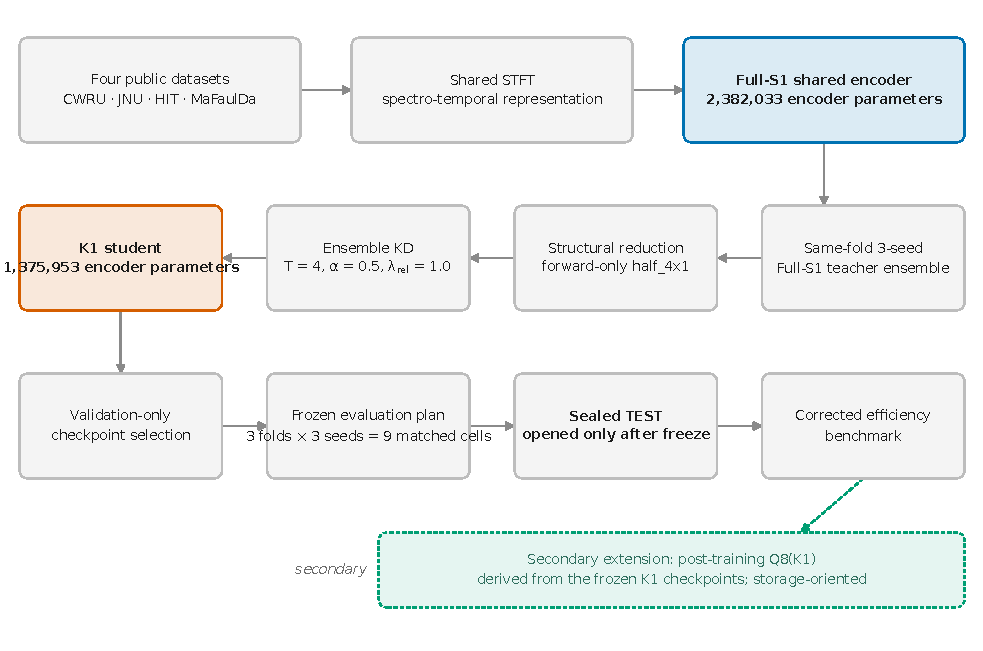
\includegraphics[width=\textwidth]{figures/fig01_workflow_overview.pdf}
  \caption{Overview of the frozen study workflow. One shared PC-STE encoder is
  trained across CWRU, JNU, HIT and MaFaulDa through a common spectro-temporal
  representation. The bidirectional Full-S1 encoder is structurally reduced to
  the forward-only K1 student, which is distilled from a same-fold ensemble of
  three independently seeded Full-S1 teachers. Checkpoints are selected on
  validation data only, and the sealed TEST partition was opened once, after the
  evaluation plan had been frozen. The post-training Q8(K1) stage (dashed) is a
  secondary, storage-oriented extension derived from the frozen K1 checkpoints
  and is not part of the primary comparison.}
  \label{fig:workflow}
\end{figure}


\subsection{Study Overview and Problem Formulation}
\label{subsec:overview}

Let $\mathcal{D}=\{\text{CWRU},\text{JNU},\text{HIT},\text{MaFaulDa}\}$ denote the four diagnostic datasets. A single encoder $E_{\theta}$ maps the representation of a vibration window to a global embedding $z\in\mathbb{R}^{192}$. Each dataset $d\in\mathcal{D}$ has a separate linear classification head $h_d$, so the encoder parameters are shared while the output label spaces remain dataset-specific:
\begin{equation}
    \hat{y}_d = h_d\!\left(E_{\theta}(x_d)\right).
\end{equation}
This design avoids forcing incompatible class taxonomies into one output head. CWRU, JNU, HIT, and MaFaulDa therefore contribute to a common representation while preserving their own labels.

Full-S1 is the reference model. It uses the full bidirectional PC-STE encoder initialized from masked-reconstruction self-supervision. K1 is the lightweight student. It retains the same embedding width, patch stem, coordinate encoder, four temporal stages, cross-band mixer, validity-aware pooling, and dataset-specific heads, but each bidirectional temporal layer is replaced by its forward-only counterpart. Q8(K1) is a deterministic post-training quantized representation of K1 and is evaluated as a secondary deployment extension.

\begin{table}[t]
\centering
\caption{Full-S1 and K1 architecture summary. The student preserves model width and temporal depth while removing the reverse state-space direction.}
\label{tab:model_architecture}
\small
\begin{tabular}{lcc}
\toprule
Property & Full-S1 & K1 \\
\midrule
Shared embedding width & 192 & 192 \\
Temporal stages & 4 & 4 \\
Directions per stage & 2 (forward + backward) & 1 (forward) \\
Mamba inner width & 384 & 384 \\
State dimension & 16 & 16 \\
Patch size (frequency $\times$ time) & $16\times8$ & $16\times8$ \\
Dataset-specific heads & 4 & 4 \\
Encoder parameters & 2,382,033 & 1,375,953 \\
Complete-model parameters & 2,385,893 & 1,379,813 \\
\bottomrule
\end{tabular}
\end{table}


The central hypothesis concerns retention rather than raw superiority: after structural reduction and distillation, K1 should not lose more than a prespecified amount of aggregate diagnostic performance relative to Full-S1. Computational measurements are conducted separately from the predictive evaluation so that inference efficiency cannot influence model selection.

\subsection{Datasets and Experimental Protocol}
\label{subsec:datasets}

The final study uses four public rotating-machinery datasets with different sampling rates, machinery configurations, and label spaces: CWRU~\citep{CWRUDataset}, JNU~\citep{JNUDataset}, HIT~\citep{Hou2023HIT}, and MaFaulDa~\citep{MaFaulDaDataset}. Table~\ref{tab:datasets} summarizes the role of each dataset. Raw signals remain at their native sampling rates; the final CWRU protocol uses official native 12~kHz recordings only and does not mix in the 48~kHz files. JNU and MaFaulDa are sampled at 50~kHz, while HIT is sampled at 25~kHz. Dataset source material is retained under the terms of the original providers.

\begin{table}[t]
\centering
\caption{Datasets and frozen evaluation principles used in the publication study. The protocols are designed to prevent direct window leakage but do not establish unseen-machine generalization.}
\label{tab:datasets}
\small
% ragged-right X columns: justified narrow cells produced visibly stretched
% inter-word gaps in the MaFaulDa row.
\begin{tabularx}{\textwidth}{l c c >{\raggedright\arraybackslash}X >{\raggedright\arraybackslash}X}
\toprule
Dataset & Classes & Native rate & Split principle & Scope of claim \\
\midrule
CWRU & 3 & 12 kHz & TRAIN: 0+1 hp; validation: 2 hp; TEST: 3 hp & Cross-load on the same rig, not cross-machine \\
JNU & 4 & 50 kHz & Guarded temporal split within frozen recordings & Held-out windows/segments, not unseen-machine \\
HIT & 3 & 25 kHz & Frozen logical-recording split & Held-out recordings under the registered protocol \\
MaFaulDa & 10 & 50 kHz & Grouped by configuration/severity & Held-out grouped conditions on the same simulator \\
\bottomrule
\end{tabularx}
\end{table}


All models operate on one-second windows. Training uses overlapping windows with a 0.5-s stride, while validation and TEST use a 1.0-s stride. The split definitions were frozen before the publication comparison. CWRU uses a load partition in which 0 and 1~hp form TRAIN, 2~hp forms validation, and 3~hp forms TEST. This evaluates cross-load behaviour on the same experimental rig; it is not an unseen-machine test. JNU uses a guarded temporal split within the available recordings, HIT uses a frozen logical-recording split rather than adopting an uncontrolled random window split, and MaFaulDa uses grouped assignments by machine configuration/severity. These protocols reduce direct window leakage, but none establishes transfer to a completely unseen machine or acquisition system. Accordingly, no cross-machine generalization claim is made.

The final design contains three global folds and three random seeds, $s\in\{42,1337,2026\}$, for nine matched cells. Within a cell $(f,s)$, Full-S1 and K1 are compared using the same fold definition and corresponding seed. TEST data are excluded from model training and validation-based checkpoint selection.

\subsection{Spectro-Temporal Input Representation}
\label{subsec:representation}

Each one-second vibration window is transformed to the frozen N2 magnitude short-time Fourier transform (STFT) representation. The transformation is performed at the dataset's native sampling rate and followed by a $\log(1+x)$ magnitude transform. The N2 configuration was selected before the final publication comparison and then held fixed. The representation stores both the spectral values and their physical frequency and time coordinates, allowing the same encoder to operate on grids arising from different native sampling rates without introducing a dataset-specific encoder branch.

Normalization is fitted on TRAIN only for every fold and dataset. The standard deviation denominator is lower-bounded by 0.05 to prevent unstable scaling of near-constant cells. The fitted normalizer is then frozen and reused for validation and TEST. When tensor completion is required for batching or patchification, padded cells are zero-filled and explicitly masked; no interpolation is used to fabricate unobserved frequency content.

PC-STE divides each spectrogram into $16\times8$ time--frequency patches. A patch stem applies a $3\times3$ convolution with eight channels and GELU activation inside each patch, followed by a linear projection to $d_{\mathrm{model}}=192$. The model additionally computes physical patch centres in kHz and seconds from valid cells only. Fourier coordinate features derived from these absolute physical coordinates are projected into the model width and added to the patch embeddings. Thus, positional information represents physical frequency and time rather than only grid indices.

\subsection{Full PC-STE and Self-Supervised Initialization}
\label{subsec:fullpcste}

The full encoder contains four temporal layers. Within each frequency band, patch tokens are processed along time by independently parameterized forward and backward Mamba blocks. For an input sequence $X$, one bidirectional layer can be written as
\begin{equation}
    Y = X + \frac{1}{2}\left[
    \mathcal{M}_{\mathrm{fwd}}(\mathrm{LN}(X)) +
    \mathrm{flip}\left(\mathcal{M}_{\mathrm{bwd}}(\mathrm{flip}(\mathrm{LN}(X)))\right)
    \right],
\end{equation}
where $\mathcal{M}$ is a Mamba-1 selective state-space block. In the implementation, $d_{\mathrm{inner}}=384$, $d_{\mathrm{state}}=16$, the depthwise causal convolution has width four, and the time-step projection rank is $\lceil192/16\rceil=12$. The official fused Mamba CUDA implementation was unavailable on the experimental software stack; therefore, the same Mamba-1 recurrence is executed in pure PyTorch. This changes implementation speed but not the model equations.

After the temporal backbone, valid tokens are averaged within each frequency band. An Hz-aware cross-band mixer computes data-dependent interactions using both the band summaries and their physical frequency features. Finally, validity-masked pooling across bands produces the shared 192-dimensional embedding consumed by the four dataset heads. The encoder has 2,382,033 trainable parameters; including the heads, the complete Full-S1 model contains 2,385,893 parameters.

Full-S1 is initialized through masked spectrogram reconstruction. During self-supervised training, 60\% of valid patches are selected by the frozen random-mask geometry and reconstruction loss is evaluated on the masked content. Training uses AdamW with learning rate $3\times10^{-4}$, betas $(0.9,0.95)$, weight decay 0.05, gradient clipping at global norm 1.0, five warm-up epochs, and cosine decay to $10^{-6}$. Self-supervised training runs for 60 epochs. The resulting encoder initializes the supervised Full-S1 models; downstream training uses the same optimizer family for 50 epochs, with validation-only checkpoint selection.

\subsection{K1 Structural Compression}
\label{subsec:k1}

K1 has the registered architecture name \texttt{half\_4x1}. The compression operation is deliberately narrow: each of the four bidirectional temporal layers is replaced by a forward-only layer while all four temporal stages are retained. If $F_l$ and $B_l$ denote the forward and backward Mamba blocks at layer $l$, Full-S1 uses both directions whereas K1 keeps $F_l$ only:
\begin{align}
  \text{Full-S1: } & X_{l+1}=X_l+\tfrac{1}{2}\left(F_l(\mathrm{LN}(X_l))+B_l^{\leftarrow}(\mathrm{LN}(X_l))\right), \\
  \text{K1: } & X_{l+1}=X_l+F_l(\mathrm{LN}(X_l)).
\end{align}
The registered residual convention is \texttt{mean\_of\_remaining}, which gives the retained branch unit residual scale rather than preserving the previous factor of one half.

K1 is constructed by deterministic surgery from the matched Full-S1 checkpoint in the same fold--seed cell. The patch stem, coordinate encoder, forward Mamba parameters, final temporal normalization, cross-band mixer, and dataset heads are copied from the teacher-side model; reverse-direction parameters are dropped. This produces a 1,375,953-parameter shared encoder and a 1,379,813-parameter complete model. Because the hidden width and number of temporal stages are unchanged, the comparison isolates directionality reduction more directly than a wholesale redesign of the student.

\subsection{Ensemble Knowledge Distillation}
\label{subsec:distillation}

For each fold $f$, the teacher set comprises the three independently seeded Full-S1 checkpoints from that fold:
\begin{equation}
  \mathcal{T}_f = \{T_{f,42},T_{f,1337},T_{f,2026}\}.
\end{equation}
Cross-fold teacher mixing is forbidden. Teacher inference is deterministic, and only TRAIN and validation outputs are cached for distillation; TEST outputs never enter K1 training.

For a dataset with class logits $z_k$ from teacher $k$, the classification soft target is the mean of the temperature-scaled teacher probabilities:
\begin{equation}
  \bar{p}_T = \frac{1}{3}\sum_{k=1}^{3}\mathrm{softmax}\left(\frac{z_k}{T}\right),
  \qquad T=4.
\end{equation}
The student classification loss combines hard-label cross-entropy and forward KL divergence from the ensemble target to the student distribution:
\begin{equation}
\mathcal{L}_{\mathrm{KD}}=
(1-\alpha)\,\mathcal{L}_{\mathrm{CE}}+
\alpha T^2\,D_{\mathrm{KL}}\!\left(\bar{p}_T\,\|\,p_s^T\right),
\qquad \alpha=0.5.
\end{equation}
A relational term aligns cross-band attention distributions between K1 and the same-cell Full-S1 teacher. Invalid or padded bands are excluded before the distributions are renormalized. The final registered loss adds this term with weight $\lambda_{\mathrm{rel}}=1.0$. Losses are first averaged over windows within each dataset and then averaged equally across datasets, ensuring that datasets with more windows do not dominate an optimization step.

K1 is trained for 50 epochs using the frozen AdamW recipe described above. The effective batch is 64 windows, organized as 16 windows per dataset. Checkpoint selection uses the maximum validation Macro-4 Macro-F1 (recorded in the frozen artifacts as \texttt{macro\_domain\_f1}) under strict improvement; exact ties retain the earlier epoch. There is no early stopping and no TEST-based model selection.

\subsection{Secondary Q8 Quantization Extension}
\label{subsec:q8}

Q8 is evaluated only after the Full-S1--K1 study and the primary efficiency benchmark were complete. It is therefore a secondary deployment extension rather than an arm of the original confirmatory comparison. Each of the nine frozen K1 \texttt{best.pt} checkpoints is converted deterministically, without retraining, fine-tuning, or calibration.

The registered accuracy representation applies per-output-channel symmetric 8-bit quantization to 23 allowlisted linear modules. For output channel $c$, the weight scale is
\begin{equation}
  s_c=\frac{\max_j |w_{c,j}|}{127}, \qquad
  q_{c,j}=\mathrm{clip}\left(\mathrm{round}(w_{c,j}/s_c),-127,127\right).
\end{equation}
The stored compact state retains the integer weights and scales, whereas evaluation of the registered \texttt{sim} representation dequantizes these weights to FP32 for computation. The time-step projection, state parameters $A_{\log}$ and $D$, depthwise convolution, layer normalizations, patch-stem convolution, and selective-scan recurrence remain FP32. Overall, 1,322,816 of 1,379,813 parameters (95.87\%) are stored as int8 weights in the quantized plan.

A separate \texttt{cpu\_dynamic} representation uses \texttt{torch.ao} dynamic quantization with the \texttt{fbgemm} backend, adding dynamic activation quantization for the same allowlisted linear layers. This is the CPU deployment representation used for runtime measurement. It is not numerically identical to \texttt{sim}; therefore, the Q8 TEST non-inferiority statement applies only to \texttt{sim}. The preserved implementation provides no true INT8 CUDA execution path, so no Q8 GPU latency or GPU-memory claim is made.

\subsection{Evaluation Metrics and Statistical Analysis}
\label{subsec:stats}

For each dataset, the evaluation records accuracy, balanced accuracy, macro precision, macro recall, Macro-F1, one-vs-rest Macro-AUC, classwise precision/recall/F1, and the confusion matrix. The primary publication endpoint is equal-domain Macro-4 Macro-F1,
\begin{equation}
  F_{\mathrm{M4}} = \frac{1}{4}\sum_{d\in\mathcal{D}}F_{1,d},
\end{equation}
so that every dataset contributes equally regardless of its number of windows. Macro-4 Macro-AUC is a secondary aggregate endpoint and is computed analogously when all four dataset AUC values are finite.

The experimental unit for the primary comparison is the matched fold--seed cell. For cell $i$, the paired difference is
\begin{equation}
  \Delta_i = F_{\mathrm{M4},i}^{\mathrm{K1}} - F_{\mathrm{M4},i}^{\mathrm{Full-S1}},
  \qquad i=1,\ldots,9.
\end{equation}
The largest acceptable Macro-F1 loss was fixed at $m=0.02$ before the final sealed TEST evaluation was run; it was not chosen after any TEST outcome had been observed. The non-inferiority hypothesis is
\begin{equation}
  H_0:\mathbb{E}[\Delta]\leq -m, \qquad
  H_1:\mathbb{E}[\Delta]>-m, \qquad m=0.02.
\end{equation}
The exact one-sided test is performed by first shifting each paired difference by the margin, $\Delta_i'=\Delta_i+m$, then enumerating all $2^9=512$ sign-flip patterns. Non-inferiority passes only when the exact one-sided $p$-value is below 0.05 and the observed shifted mean is positive. A two-sided exact superiority test is reported only after the non-inferiority gate passes, and is treated as supportive secondary evidence rather than the primary study claim. Descriptive dispersion is the sample standard deviation across all nine cells.

For Q8, the paired unit is again fold--seed, but the historical quantization margin is $-0.01$ and the contrast is Q8 minus K1. The exact one-sided sign-flip procedure is reused without adding a superiority test. Because the broader historical multiple-hypothesis family was not executable in the publication extension, the Q8 contrast is reported as a standalone secondary analysis without family-wise multiplicity adjustment.

\subsection{Computational Efficiency Evaluation}
\label{subsec:efficiency_method}

Model complexity is characterized by encoder and complete-model parameter counts, standardized FP32 state-dictionary size, FLOPs per one-second window, batch-1 latency, batch-32 throughput, and GPU peak allocated memory. FLOPs combine a dense-operator count with an analytic selective-scan term; the same convention is applied to both Full-S1 and K1. Because CWRU uses a smaller native-12~kHz spectrogram grid than the historical mixed-rate implementation, the scan term uses the final publication representation rather than the superseded mixed-rate band count.

Runtime measurement uses one deterministically fixed representative pair, global fold 1 / seed 42, selected by the rule ``lowest fold, then lowest seed'' before any efficiency outcome was observed. The first validation window in frozen manifest order is used for each dataset, and the same inputs are supplied to both models. Measurements were obtained on an idle Intel Core i9-14900 host with an NVIDIA RTX 4000 Ada Generation GPU, PyTorch 2.12.0+cu130, and CUDA 13.0. CPU timing uses one thread.

The authoritative timing correction runs both models in evaluation mode with PyTorch inference mode explicitly verified inside the timed loop. CPU batch-1 measurements use 100 warm-up and 1000 timed iterations per dataset and scope; GPU batch-1 uses 200 warm-up and 1000 timed iterations with synchronization. Model-only latency measures prepared representation to logits, while end-to-end latency additionally includes STFT construction and normalization but excludes disk I/O. Batch-32 throughput is measured separately. Full-S1 and K1 are interleaved to reduce temporal bias, and the headline value is the equal-domain mean of the four per-dataset medians. All latency measurements use the pure-PyTorch selective scan rather than a fused Mamba kernel, so absolute times should be interpreted for this software stack rather than as hardware-independent constants.

\section{Results and Discussion}
\label{sec:results}

The results are presented in the same order as the scientific question. First, the sealed matched TEST comparison establishes whether K1 retains Full-S1 diagnostic performance. Second, dataset-level behaviour is examined to identify where the aggregate difference arises, and the pooled confusion matrices localize it to individual classes. Third, the prespecified non-inferiority result is interpreted using the nine paired cells. Structural efficiency and the secondary Q8 extension are then considered to determine what is gained in deployment terms, before the work is positioned against related approaches and its limitations are stated.

\subsection{Full-S1 versus K1 Diagnostic Performance}
\label{subsec:main_results}

\begin{table}[t]
\centering
\caption{Final sealed Full-S1 versus K1 aggregate results across nine matched fold--seed cells. Values are mean $\pm$ sample SD.}
\label{tab:main_results}
\small
\begin{tabular}{lccc}
\toprule
Endpoint & Full-S1 & K1 & Paired $\Delta$ (K1--Full-S1) \\
\midrule
Macro-4 Macro-F1 & $0.934644 \pm 0.023258$ & $0.955334 \pm 0.018393$ & $+0.020691 \pm 0.013509$ \\
Macro-4 Macro-AUC & $0.991793 \pm 0.008102$ & $0.996398 \pm 0.002367$ & $+0.004606 \pm 0.006794$ \\
\bottomrule
\end{tabular}
\end{table}

\begin{table}[t]
\centering
\caption{Macro-4 Macro-F1 in the nine matched fold--seed TEST cells.}
\label{tab:matched_cells}
\small
\begin{tabular}{ccrrr}
\toprule
Fold & Seed & Full-S1 & K1 & $\Delta$ (K1--Full-S1) \\
\midrule
1 & 42   & 0.932734 & 0.944172 & +0.011438 \\
1 & 1337 & 0.953079 & 0.950776 & -0.002303 \\
1 & 2026 & 0.926615 & 0.941293 & +0.014678 \\
2 & 42   & 0.947566 & 0.977788 & +0.030222 \\
2 & 1337 & 0.943998 & 0.972982 & +0.028984 \\
2 & 2026 & 0.879871 & 0.919195 & +0.039324 \\
3 & 42   & 0.957175 & 0.967335 & +0.010160 \\
3 & 1337 & 0.926540 & 0.961007 & +0.034467 \\
3 & 2026 & 0.944214 & 0.963463 & +0.019249 \\
\bottomrule
\end{tabular}
\end{table}

% Figure 2 — matched fold-seed performance.
% Asset generated by scripts/publication_figures/fig02_matched_cells.py
\begin{figure}[tb]
  \centering
  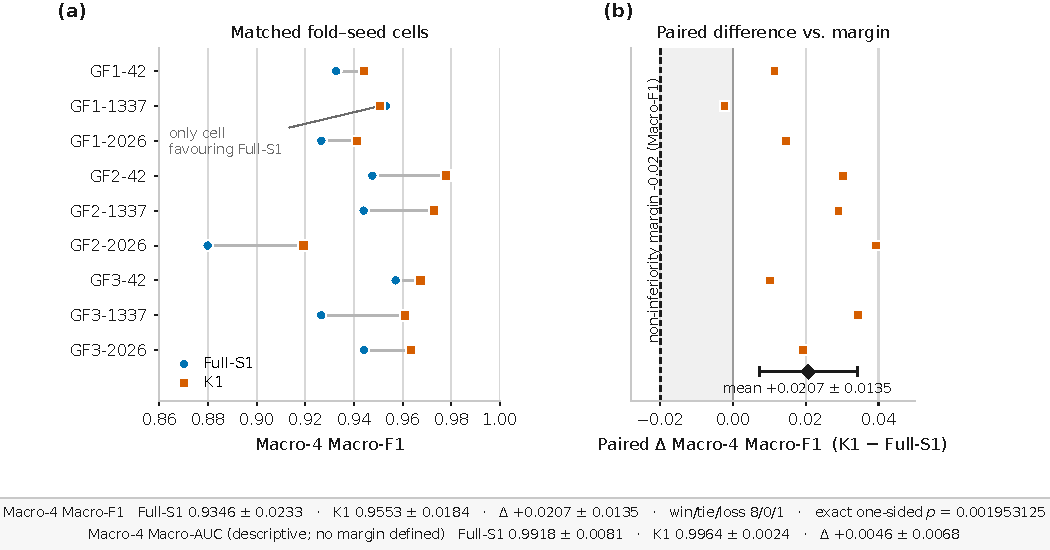
\includegraphics[width=\textwidth]{figures/fig02_matched_cells.pdf}
  \caption{Matched fold--seed comparison of Full-S1 and K1 on the sealed TEST
  partition. (a) Macro-4 Macro-F1 in each of the nine matched cells, with the
  connecting segment showing the paired change. (b) The nine paired differences
  relative to the prespecified $-0.02$ Macro-F1 non-inferiority margin (dashed);
  the diamond marks the mean $\pm$ sample SD of the paired difference. The
  margin was defined for Macro-F1 only: the Macro-AUC values quoted below the
  panels are descriptive, and no non-inferiority margin was specified for them.}
  \label{fig:matched_cells}
\end{figure}


Table~\ref{tab:main_results} summarizes the primary sealed TEST result. Full-S1 obtains a Macro-4 Macro-F1 of $0.934644\pm0.023258$, whereas K1 obtains $0.955334\pm0.018393$. The mean paired change is therefore $+0.020691\pm0.013509$. Eight of the nine matched fold--seed cells favour K1 and one favours Full-S1. Macro-4 Macro-AUC follows the same overall direction, increasing from $0.991793\pm0.008102$ to $0.996398\pm0.002367$ with a paired mean change of $+0.004606\pm0.006794$.

The cell-level values in Table~\ref{tab:matched_cells}, plotted in Figure~\ref{fig:matched_cells}, are important because the aggregate mean does not arise from one isolated run. Positive K1 Macro-F1 differences occur in all three folds, and the largest gain appears in fold 2 / seed 2026 ($+0.039324$). The only negative Macro-F1 cell is fold 1 / seed 1337 ($-0.002303$), a magnitude far inside the predefined acceptable-loss margin. This paired pattern supports the interpretation that K1's performance retention is reproducible across the registered fold--seed design rather than being attributable to a single selected checkpoint.

The observed mean is higher for K1, but the study was designed as a non-inferiority experiment rather than a universal superiority claim. The result therefore supports the narrower conclusion that substantial structural reduction was achieved without an unacceptable aggregate performance loss. The positive point estimate and the gated superiority test are useful additional evidence, but they do not imply that K1 must outperform Full-S1 for every dataset, fold, seed, or future operating condition.

\subsection{Dataset-Level Performance}
\label{subsec:dataset_results}

\begin{table}[t]
\centering
\caption{Dataset-level Macro-F1 for Full-S1 and K1. Values are mean $\pm$ sample SD across the nine matched cells.}
\label{tab:dataset_results}
\small
\begin{tabular}{lccc}
\toprule
Dataset & Full-S1 & K1 & Paired $\Delta$ \\
\midrule
CWRU & $0.854747 \pm 0.083579$ & $0.918945 \pm 0.073432$ & $+0.064198 \pm 0.044152$ \\
JNU & $0.971429 \pm 0.042857$ & $0.980952 \pm 0.037796$ & $+0.009524 \pm 0.028571$ \\
HIT & $0.991039 \pm 0.017798$ & $0.988728 \pm 0.016133$ & $-0.002311 \pm 0.007427$ \\
MaFaulDa & $0.921360 \pm 0.016432$ & $0.932712 \pm 0.017321$ & $+0.011352 \pm 0.019450$ \\
\bottomrule
\end{tabular}
\end{table}

\begin{table}[t]
\centering
\caption{Dataset-level Macro-AUC for Full-S1 and K1. Values are mean $\pm$ sample SD across the nine matched cells. Dataset-level values are descriptive rather than separate confirmatory tests.}
\label{tab:dataset_results_auc}
\small
\begin{tabular}{lccc}
\toprule
Dataset & Full-S1 & K1 & Paired $\Delta$ \\
\midrule
CWRU & $0.974093 \pm 0.033643$ & $0.990379 \pm 0.009921$ & $+0.016286 \pm 0.027983$ \\
JNU & $0.999559 \pm 0.001323$ & $1.000000 \pm 0.000000$ & $+0.000441 \pm 0.001323$ \\
HIT & $0.999969 \pm 0.000094$ & $0.999602 \pm 0.001082$ & $-0.000366 \pm 0.001095$ \\
MaFaulDa & $0.993549 \pm 0.006247$ & $0.995611 \pm 0.004732$ & $+0.002062 \pm 0.003131$ \\
\bottomrule
\end{tabular}
\end{table}

% Figure 3 — dataset-level performance.
% Asset generated by scripts/publication_figures/fig03_dataset_level.py
\begin{figure}[tb]
  \centering
  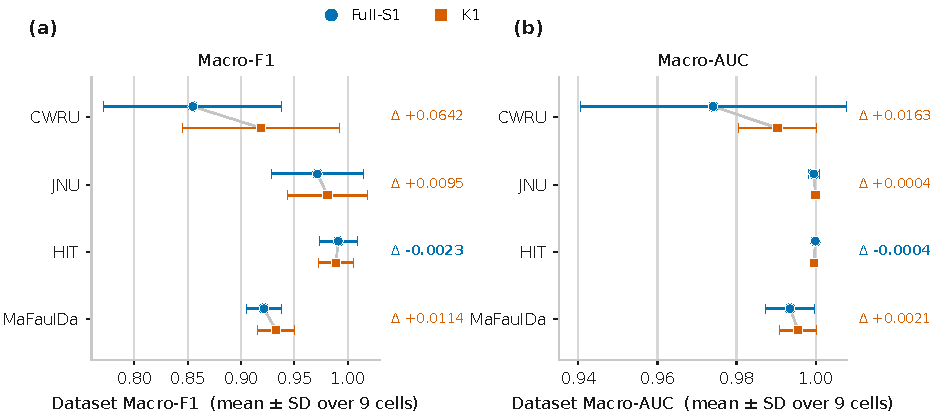
\includegraphics[width=\textwidth]{figures/fig03_dataset_level.pdf}
  \caption{Dataset-level performance of Full-S1 and K1: (a) Macro-F1 and
  (b) Macro-AUC, each shown as the mean over the nine matched fold--seed cells
  with sample-SD whiskers. $\Delta$ is the paired mean difference
  (K1 $-$ Full-S1). HIT is the only dataset whose mean decreases under K1, on
  both endpoints. Dots rather than bars are used because both axes are
  truncated and do not begin at zero.}
  \label{fig:dataset_level}
\end{figure}


Figure~\ref{fig:dataset_level} shows both endpoints per dataset. The largest dataset-level change occurs on CWRU, where mean Macro-F1 increases from $0.854747$ to $0.918945$, a paired improvement of $+0.064198$. CWRU is also the dataset with the largest between-cell variability for both models. This is consistent with the observation that its fault categories remain more sensitive to the chosen split and seed than the near-saturated JNU and HIT tasks. The corresponding CWRU Macro-AUC increases by $+0.016286$.

JNU shows a smaller positive mean change in Macro-F1 ($+0.009524$). Eight of the nine JNU cells are ties at the reported precision and one favours K1, while the mean Macro-AUC changes from $0.999559$ to $1.000000$. This near-ceiling behaviour limits the amount of improvement that can be expressed numerically. MaFaulDa also improves on average, with Macro-F1 increasing by $+0.011352$ and Macro-AUC by $+0.002062$. Because MaFaulDa contains ten classes and a wider variety of machine conditions, preserving or improving its performance after structural reduction is particularly relevant to the claim that one compact encoder can continue to serve heterogeneous label spaces.

HIT is the exception to the otherwise positive dataset means. Its Macro-F1 decreases slightly from $0.991039$ to $0.988728$ ($-0.002311$), and Macro-AUC decreases by $-0.000366$. The absolute level remains high, but this negative delta is important because it prevents the aggregate result from being interpreted as universal dominance. K1's benefit is therefore best described as retained aggregate performance with favourable mean behaviour on three datasets, rather than guaranteed improvement on every constituent domain.

The class-level reports stored with the frozen evaluation further show that the weaker CWRU behaviour is concentrated in confusions among bearing-fault categories rather than a collapse of the entire representation; Section~\ref{subsec:confusion_analysis} examines this structure directly. These class-level differences motivate future work on stronger inter-class separation, but they do not change the main compression result: K1 retains the multi-dataset diagnostic role while using substantially fewer temporal-direction parameters.

\subsection{Aggregated Confusion-Matrix Analysis}
\label{subsec:confusion_analysis}

% -----------------------------------------------------------------------------
% Aggregated confusion-matrix figure (Full-S1 vs K1).
%
% Asset: figures/fig_confusion_aggregated_fulls1_vs_k1.pdf
%   natural size 7.16in x 8.71in, vector, generated by
%   scripts/generate_confusion_figure.py in the publication repository.
%   Provenance and verification:
%   figures/confusion_matrices/confusion_matrix_aggregation_manifest.md
%
% A plain `figure' float is used: the manuscript is single-column, so figure*
% gains nothing here and a separate float class would not be guaranteed to keep
% its numbering position relative to the other figures. Switch to figure* if the
% manuscript is migrated to a two-column journal class.
% keepaspectratio with a height cap leaves room for the caption and lets the
% float shrink for classes with a shorter text block; it does not bind here.
% -----------------------------------------------------------------------------
\begin{figure}[p]
  \centering
  \includegraphics[width=\textwidth,height=0.78\textheight,keepaspectratio]%
    {figures/fig_confusion_aggregated_fulls1_vs_k1.pdf}
  \caption{Aggregated class-level confusion matrices for Full-S1 (left column)
  and K1 (right column) on the four evaluation datasets: CWRU, JNU, HIT and
  MaFaulDa. For each dataset and model, the raw confusion counts of the nine
  matched fold--seed evaluation cells were summed element-wise, and the pooled
  matrix was then normalized by true class; each row therefore shows the
  distribution of predictions conditional on the true class, and all panels
  share the same $0$--$100\%$ colour scale; exactly-zero cells are left blank.
  The pooled matrices are descriptive summaries of the nine matched model
  evaluations rather than a single independent test split; all inferential
  comparisons rest on the paired fold--seed analysis reported in
  Section~\ref{subsec:ni_results}.}
  \label{fig:confusion_aggregated}
\end{figure}


The dataset-level scores above establish that K1 retains the predictive
behaviour of Full-S1, but they do not localize where the two models differ.
Figure~\ref{fig:confusion_aggregated} provides that view. For each dataset and
model, the raw confusion counts of the nine matched fold--seed cells were summed
element-wise and the pooled matrix was then normalized by true class, so that
each row shows the distribution of predictions conditional on the true class.
These matrices are descriptive summaries of the nine matched evaluations rather
than an additional inferential test; the retention claim continues to rest on
the paired analysis reported in Section~\ref{subsec:ni_results}.

The clearest difference appears on CWRU, the dataset with the largest paired
Macro-F1 improvement. Recall of the \texttt{inner\_race} class rises from
approximately $77.3\%$ to $84.6\%$, while the dominant off-diagonal term,
\texttt{inner\_race} predicted as \texttt{outer\_race}, falls from roughly
$20.6\%$ to $15.2\%$. This reduction in inner-/outer-race confusion is
consistent with, and likely contributes to, the improved CWRU Macro-F1 of K1.
It also makes the preceding qualitative statement concrete: the weaker CWRU
behaviour of Full-S1 is concentrated in one specific race-fault confusion rather
than distributed across the three-class CWRU label space.

JNU and HIT are near-diagonal for both models, consistent with their near-ceiling
dataset-level scores. For JNU the pooled sample count is small ($n=216$ across
all nine cells), so a single window shifts a row entry by several percentage
points and the small differences visible between the two columns should not be
over-interpreted. HIT is informative for the opposite reason: it is the one
dataset whose mean Macro-F1 decreases under K1, and the pooled matrices localize
that decrease to class~1, the inner-ring fault condition, whose recall moves
from about $97.3\%$ to $96.6\%$. The class-level evidence therefore supports the
non-inferiority reading developed in Section~\ref{subsec:ni_results}, in which
compression leaves already-strong behaviour essentially intact, rather than a
claim that K1 improves on every dataset and every class.

MaFaulDa remains the most fine-grained task, and its panels show that the
residual errors stay localized to a small number of physically adjacent class
pairs rather than spreading across the ten-class label space. The most
persistent of these is the confusion between \texttt{overhang/cage\_fault} and
\texttt{overhang/outer\_race}, which is almost unchanged between the two models:
$11.5\%$ of true \texttt{overhang/cage\_fault} windows are assigned to
\texttt{overhang/outer\_race} under both Full-S1 and K1, and the reverse
confusion moves only from $19.4\%$ to $17.4\%$. That this pattern survives
compression largely intact suggests that it is intrinsic to the dataset rather
than induced by the reduced model. Taken together, the class-level analysis
supports the view that the performance retention of K1 is not an artefact of
scalar summaries: the lightweight model preserves the qualitative error
structure of the Full-S1 baseline and, on CWRU in particular, reduces one of its
most persistent confusion patterns.

\subsection{Performance Retention and Non-Inferiority}
\label{subsec:ni_results}

The predefined primary margin was $-0.02$ Macro-F1. The observed mean paired difference, $+0.020691$, is therefore $0.040691$ above the non-inferiority boundary after margin shifting. Exact enumeration of all 512 sign patterns gives a one-sided non-inferiority $p$-value of $0.001953125$, the minimum attainable value with nine matched cells under this procedure. The non-inferiority criterion is consequently satisfied.

Because the non-inferiority gate passed, the frozen analysis also reports a two-sided exact sign-flip test for superiority, yielding $p=0.0078125$. This secondary result is supportive, but it should be interpreted in the context of the small number of paired units and the study's original objective. No confidence interval for the paired difference was pre-registered, and none is introduced post hoc as a confirmatory quantity. The strongest statistically aligned statement is therefore that K1 is non-inferior to Full-S1 at the predefined $-0.02$ Macro-F1 margin.

The paired design is important for this conclusion. Rather than comparing two independently averaged collections of runs, each K1 outcome is linked to a Full-S1 outcome from the same global fold and seed. The resulting $\Delta_{f,s}$ values partially control fold and stochastic-training variability and make the sign-flip test operate on the same experimental units that generated the models. This is a more direct measure of compression retention than comparing two unpaired grand means.

\subsection{Computational Efficiency}
\label{subsec:efficiency_results}

\begin{table}[t]
\centering
\caption{Authoritative publication efficiency comparison. Latency/throughput values use the corrected inference-mode benchmark.}
\label{tab:efficiency}
\small
\begin{tabular}{lrrr}
\toprule
Metric & Full-S1 & K1 & Reduction / speed-up \\
\midrule
Encoder parameters & 2,382,033 & 1,375,953 & 42.24\% \\
FP32 state-dict size & 9.135 MiB & 5.286 MiB & 42.14\% \\
Macro-4 computation & 2.6067 GFLOP & 1.4236 GFLOP & 45.38\% \\
CPU b1 model-only & 54.709 ms & 28.560 ms & 1.916$\times$ \\
CPU b1 end-to-end & 55.699 ms & 29.725 ms & 1.874$\times$ \\
GPU b1 model-only & 7.711 ms & 4.164 ms & 1.852$\times$ \\
GPU b1 end-to-end & 9.577 ms & 5.864 ms & 1.633$\times$ \\
GPU b32 throughput & 392.85 win/s & 785.47 win/s & 1.999$\times$ \\
CPU b32 throughput & 13.84 win/s & 26.27 win/s & 1.897$\times$ \\
GPU peak memory & 29.466 MiB & 24.823 MiB & 15.76\% \\
\bottomrule
\end{tabular}
\end{table}

% Figure 5 — computational efficiency.
% Asset generated by scripts/publication_figures/fig05_efficiency.py
\begin{figure}[!tb]
  \centering
  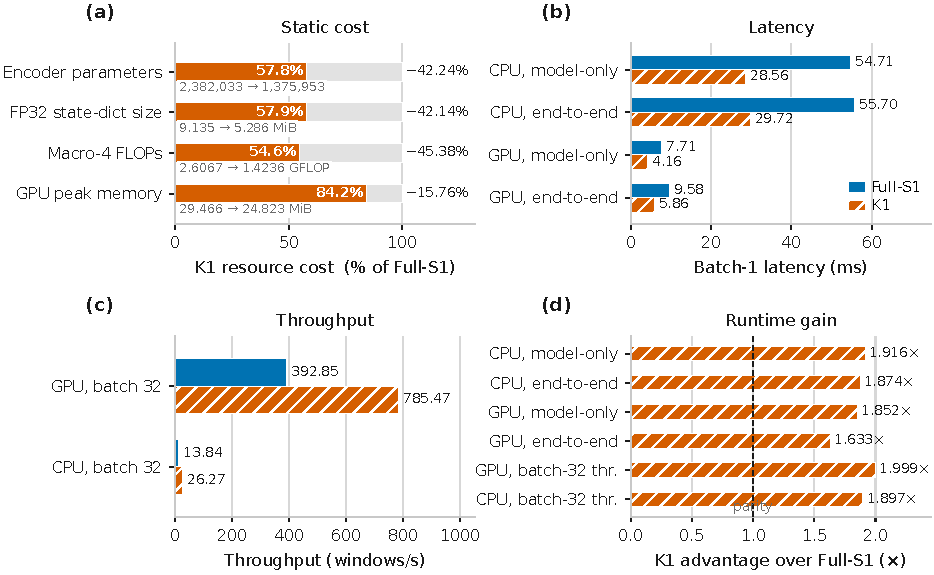
\includegraphics[width=\textwidth]{figures/fig05_efficiency.pdf}
  \caption{Computational efficiency of K1 relative to Full-S1.
  (a) Static resource cost as a percentage of Full-S1, with the absolute values
  beneath each bar. (b) Batch-1 latency for both devices and both measurement
  scopes. (c) Batch-32 throughput. (d) The K1 advantage expressed as a ratio,
  against a parity line at $1.0$. All latency and throughput values come from
  the corrected inference-mode benchmark measured on one deterministically
  selected fold--seed pair; because the selective scan is the reference
  pure-PyTorch recurrence rather than a fused kernel, absolute times are
  specific to this software stack.}
  \label{fig:efficiency}
\end{figure}


Figure~\ref{fig:efficiency} summarises the comparison. The structural change produces substantial reductions before any quantization is applied. K1 contains 1,375,953 encoder parameters compared with 2,382,033 for Full-S1, a $42.24\%$ reduction. Complete-model FP32 state-dictionary size falls by $42.14\%$, from 9.135 to 5.286~MiB. Equal-domain compute decreases by $45.38\%$, from 2.6067 to 1.4236~GFLOP per one-second window. These reductions are consistent with the design: removing one of two independently parameterized state-space directions eliminates a large part of the temporal backbone while leaving the shared stem, coordinate encoder, mixer, and heads intact.

The corrected latency benchmark shows that this reduction translates into real runtime improvements on both CPU and GPU. CPU batch-1 model-only latency decreases from 54.709 to 28.560~ms ($1.916\times$), while end-to-end latency decreases from 55.699 to 29.725~ms ($1.874\times$). GPU model-only latency falls from 7.711 to 4.164~ms ($1.852\times$), and end-to-end latency from 9.577 to 5.864~ms ($1.633\times$). At batch 32, GPU throughput is effectively doubled, from 392.85 to 785.47 windows/s, and CPU throughput increases from 13.84 to 26.27 windows/s.

GPU peak allocated memory decreases by $15.76\%$, which is smaller than the parameter-size reduction because activations and runtime buffers remain present for both models. The difference between parameter reduction and memory reduction illustrates why deployment evidence should not rely on parameter count alone.

An audit after the original efficiency run identified that the first latency/throughput timing path had omitted \texttt{torch.inference\_mode()} despite the benchmark plan stating that it should be active. The frozen historical run was preserved for provenance and a separate correction benchmark was executed on the same representative checkpoint pair and validation inputs. The corrected values in Table~\ref{tab:efficiency} are therefore the authoritative publication numbers. The correction reduced absolute latency for both models and revised the CPU speed-up from roughly $2.2\times$ to roughly $1.9\times$, while leaving the qualitative conclusion unchanged. This correction is reported because inference benchmarking is sensitive to execution context, and preserving the audit trail is preferable to silently replacing the original measurement.

The timing results should also be interpreted relative to the implementation. The selective scan is the reference pure-PyTorch recurrence rather than a fused Mamba kernel. The reported ratios are valid for the common stack used in this study, but absolute milliseconds and potentially some relative speed-ups may change under optimized kernels or different hardware. The results therefore demonstrate deployment-oriented efficiency rather than a universal hardware speed claim.

\subsection{Secondary Q8 Deployment Extension}
\label{subsec:q8_results}

\begin{table}[t]
\centering
\caption{Secondary Q8 deployment extension. The predictive non-inferiority result applies to the weight-only simulated Q8 representation, not to the CPU-dynamic deployment artifact.}
\label{tab:q8}
\small
\begin{tabular}{lrrr}
\toprule
Metric & K1 FP32 & Q8(K1) & Change \\
\midrule
Macro-4 Macro-F1 & $0.955334 \pm 0.018393$ & $0.955334 \pm 0.018405$ & $-0.0000009 \pm 0.0001101$ \\
Macro-4 Macro-AUC & $0.996398 \pm 0.002367$ & $0.996395 \pm 0.002376$ & $-0.0000031 \pm 0.0000156$ \\
Stored model size & 5.285 MiB & 1.526 MiB & $-71.12\%$ \\
CPU b1 model-only latency & 31.046 ms & 28.647 ms & 1.084$\times$ \\
CPU b32 throughput & 26.56 win/s & 27.34 win/s & 1.029$\times$ \\
Parameters & 1,379,813 & 1,379,813 & unchanged \\
\bottomrule
\end{tabular}
\end{table}

% Figure 6 — secondary Q8(K1) extension.
% Asset generated by scripts/publication_figures/fig06_q8.py
\begin{figure}[tb]
  \centering
  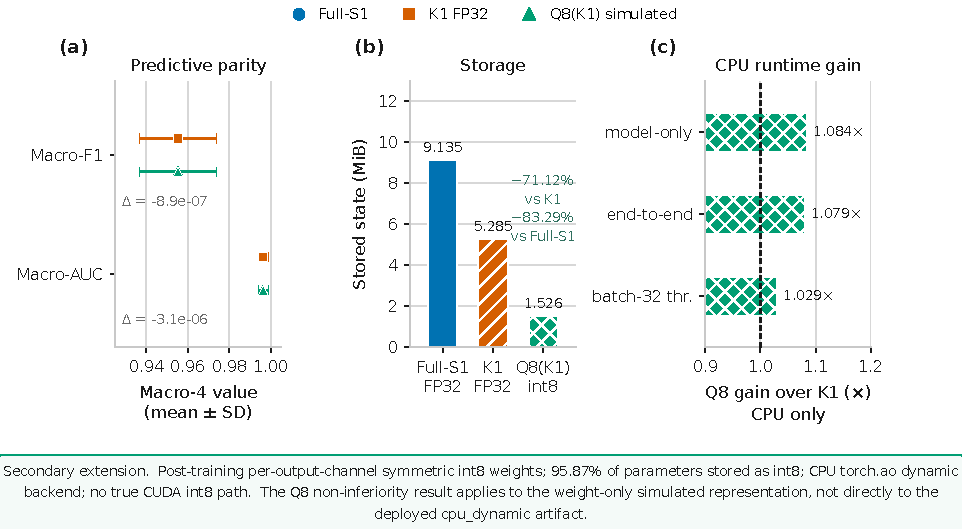
\includegraphics[width=\textwidth]{figures/fig06_q8_extension.pdf}
  \caption{Secondary Q8(K1) deployment extension. (a) The weight-only simulated
  Q8 representation matches K1 FP32 on both Macro-4 endpoints, with paired mean
  differences of order $10^{-6}$ or smaller. (b) Stored state-dictionary size
  for the representative fold--seed cell. (c) CPU runtime gain of Q8 over K1,
  measured within the Q8 benchmark, against a parity line. The predictive
  result applies to the simulated weight-only representation and does not
  transfer automatically to the deployed \texttt{cpu\_dynamic} artifact; no GPU
  int8 execution path exists on the preserved stack.}
  \label{fig:q8}
\end{figure}


Figure~\ref{fig:q8} separates the three aspects of the extension. The Q8 stage changes storage precision without changing the model architecture or parameter count. On the registered \texttt{sim} accuracy representation, Macro-4 Macro-F1 changes from $0.955334\pm0.018393$ for K1 FP32 to $0.955334\pm0.018405$ for Q8, with a mean paired difference of only $-9\times10^{-7}$. Six of nine cells are exactly tied at the reported Macro-F1 precision. The historically defined $-0.01$ non-inferiority criterion is satisfied by the same exact one-sided sign-flip procedure ($p=0.001953125$).

The principal Q8 benefit is storage. The standardized K1 state decreases from 5.285~MiB to 1.526~MiB, a $71.12\%$ reduction or $3.46\times$ compression relative to K1. Relative to Full-S1, the Q8 state is $83.29\%$ smaller, corresponding to approximately $5.99\times$ lower stored size. In contrast, runtime improvement on the real CPU dynamic-quantization backend is modest: model-only batch-1 latency improves from 31.046 to 28.647~ms ($1.084\times$), and batch-32 throughput from 26.56 to 27.34 windows/s ($1.029\times$). This difference between storage and runtime is expected because the selective-scan recurrence and several sensitive modules remain FP32.

Two boundaries are essential when interpreting Q8. First, the preserved implementation does not offer a true INT8 CUDA path. Timing the simulated representation on the GPU would therefore measure FP32 arithmetic on dequantized weights and would not constitute an INT8 acceleration result; no such claim is made. Second, the TEST accuracy evaluation applies to \texttt{sim}, whereas the CPU deployment model uses dynamic activation quantization in addition to int8 weights. On validation data, these two representations agree on 98.63\% of top-1 predictions in the equal-domain summary, but agreement falls to 95.0\% on MaFaulDa, where the maximum absolute probability difference reaches 0.49. Consequently, the formal Q8 non-inferiority result does not automatically transfer to the deployed \texttt{cpu\_dynamic} artifact. A future pre-registered evaluation of the exact deployed representation would be required to make that stronger claim.

Taken together, the three-stage result distinguishes two mechanisms. Structural compression from Full-S1 to K1 delivers most of the compute and latency reduction, whereas post-training Q8 contributes mainly a further storage reduction. This separation is useful for deployment decisions because it avoids treating weight precision and architecture size as interchangeable sources of efficiency.

\subsection{Comparison with Related Approaches}
\label{subsec:comparison}

\begin{table}[t]
\centering
\caption{Qualitative positioning against representative related work. A check mark indicates that the cited work explicitly addresses the corresponding dimension; the table is not an accuracy leaderboard.}
\label{tab:related_work}
\scriptsize
\resizebox{\textwidth}{!}{%
\begin{tabular}{lcccccccl}
\toprule
Work & Reusable / multi-dataset & Mamba/SSM & Structural compression & KD & Multi-teacher & Quantization & Physical edge & Main distinction \\
\midrule
FaultFormer \citep{Zhou2024FaultFormer} & \checkmark & -- & -- & -- & -- & -- & -- & SSL/adaptation, not deployment compression \\
BearingFM \citep{Lai2024BearingFM} & \checkmark & -- & -- & -- & -- & -- & concept & Foundation-style bearing representation \\
RmGPT \citep{Wang2025RmGPT} & \checkmark & -- & -- & -- & -- & -- & -- & Unified diagnosis/prognosis model \\
VibFM \citep{Mannone2026VibFM} & \checkmark & -- & -- & -- & -- & -- & -- & 16-dataset masked spectrogram pretraining \\
MD-BiMamba \citep{Wang2025MDBiMamba} & -- & \checkmark & -- & -- & -- & -- & -- & Bidirectional Mamba diagnosis \\
VibrMamba \citep{Yi2025VibrMamba} & multi-task & \checkmark & lightweight design & -- & -- & -- & -- & Lightweight Mamba designed directly \\
DTCP-MAKD \citep{Zhong2024DTCPMAKD} & -- & -- & \checkmark & \checkmark & assistants & -- & -- & Channel pruning + teacher assistants \\
BFD-KD \citep{Sun2026BFDKD} & -- & -- & lightweight student & \checkmark & \checkmark & -- & -- & Multi-teacher rolling-bearing KD \\
BearingPGA-Net \citep{Liao2024BearingPGANet} & -- & -- & compact student & \checkmark & -- & \checkmark & \checkmark & KD + quantization + FPGA \\
\textbf{PC-STE/K1 (this work)} & \checkmark & \checkmark & \checkmark & \checkmark & seed ensemble & Q8 secondary & -- & Shared encoder + direction reduction + paired retention test \\
\bottomrule
\end{tabular}%
}
\end{table}


Table~\ref{tab:related_work} is intended as a positioning comparison rather than a numerical leaderboard. Direct accuracy, latency, and FLOP comparisons across these papers would be misleading because datasets, split protocols, input lengths, hardware, and software kernels differ substantially. Instead, the table identifies which research dimensions each work explicitly addresses.

The closest architecture-centric comparison is VibrMamba, which establishes lightweight bidirectional Mamba-based rotating-machinery diagnosis across several classification tasks \citep{Yi2025VibrMamba}. The distinction is that K1 is obtained by compressing an already trained shared encoder and is evaluated against its own matched Full-S1 reference. MD-BiMamba establishes bidirectional Mamba processing in bearing diagnosis but does not study the same teacher-to-forward-student compression problem \citep{Wang2025MDBiMamba}. On the compression side, DTCP-MAKD and BFD-KD demonstrate structural or multi-teacher distillation strategies, but their teacher construction and model roles differ from the same-architecture seed ensemble used here \citep{Zhong2024DTCPMAKD,Sun2026BFDKD}. BearingPGA-Net provides stronger evidence of physical embedded deployment through FPGA acceleration and therefore bounds the present claim to \emph{deployment-oriented} benchmarking rather than physical edge deployment \citep{Liao2024BearingPGANet}.

Foundation-style approaches such as FaultFormer, BearingFM, RmGPT, and VibFM show that reusable or pretrained vibration representations are already established \citep{Zhou2024FaultFormer,Lai2024BearingFM,Wang2025RmGPT,Mannone2026VibFM}. PC-STE/K1 is not positioned as a larger or more general foundation model than these approaches. Its contribution is narrower: it studies how a shared multi-dataset state-space representation can be structurally compressed, distilled, and evaluated as a paired performance-retention problem with explicit computational measurement.

\subsection{Discussion and Limitations}
\label{subsec:limitations}

The result that K1's mean Macro-F1 is higher than Full-S1 may initially appear counterintuitive because K1 removes half of the directional temporal paths. One plausible explanation is that the structural reduction acts as a form of regularization while the three-teacher ensemble provides a smoother target distribution than any single teacher. Removing the reverse path may also reduce optimization burden on these relatively short patch sequences. However, the experiment was not designed to isolate these mechanisms, and the observed improvement should not be presented as proof of causality. The defensible conclusion is empirical: the removed direction was not necessary to retain aggregate performance under the registered protocol.

Several limitations bound the scope of the result. First, the four datasets provide heterogeneous benchmark conditions but do not constitute an unseen-machine evaluation. In CWRU, the final split is cross-load on the same rig; JNU and HIT similarly do not establish transfer to an entirely new machine and sensing system. The work therefore evaluates a shared multi-dataset model under frozen within-dataset protocols, not universal machinery generalization.

Second, the computational benchmark uses one deterministically selected fold--seed model pair on one workstation-class CPU/GPU system. This controls model choice and permits reproducible within-host comparisons, but it does not capture variation across embedded processors, other GPUs, or optimized inference runtimes. The pure-PyTorch selective scan is particularly relevant: a fused Mamba implementation could change absolute latency and may change the relative benefit of removing a direction.

Third, Q8 is a secondary extension with a deliberate separation between the predictive and deployed representations. The registered \texttt{sim} representation supports the non-inferiority result, whereas the actual CPU dynamic-quantization artifact has only validation-level agreement measurements. No Q8 GPU acceleration is available on the preserved stack. These constraints mean that Q8 currently supports a strong storage-compression statement and a modest CPU deployment observation, but not a fully validated INT8 edge-deployment claim.

Finally, the aggregate metric hides differences in dataset difficulty. CWRU remains substantially more variable than JNU and HIT, and some bearing-fault classes remain harder to separate. Future work should therefore investigate representations and objectives that improve class separation without sacrificing the shared-encoder design, and should extend evaluation to genuinely unseen machines or acquisition systems.

\section{Conclusion and Future Work}
\label{sec:conclusion}

This study investigated whether a shared multi-dataset selective-state-space encoder for rotating-machinery fault diagnosis can be compressed without an unacceptable loss of diagnostic performance. Rather than designing an unrelated lightweight classifier, the proposed K1 model is structurally derived from the bidirectional Full-S1 PC-STE encoder by removing the reverse selective-scan path while retaining four temporal stages, the 192-dimensional representation, physical-coordinate encoding, cross-band mixing, and dataset-specific output heads. K1 is then distilled from a same-fold ensemble of independently seeded Full-S1 teachers.

The sealed nine-cell evaluation shows that this structural reduction preserves the diagnostic role of the shared encoder. Macro-4 Macro-F1 changes from $0.934644\pm0.023258$ for Full-S1 to $0.955334\pm0.018393$ for K1, with a mean paired difference of $+0.020691\pm0.013509$. The prespecified $-0.02$ Macro-F1 non-inferiority criterion is satisfied by the exact paired sign-flip test. At the same time, K1 reduces encoder parameters by $42.24\%$, FP32 serialized size by $42.14\%$, and equal-domain computation by $45.38\%$. Under the corrected inference benchmark, K1 provides approximately $1.87\times$ CPU and $1.63\times$ GPU end-to-end batch-1 speed-ups, and nearly doubles GPU batch-32 throughput.

The secondary Q8 extension further separates storage compression from architectural acceleration. The registered simulated-Q8 representation retains essentially the same Macro-4 Macro-F1 as K1 and satisfies its historical $-0.01$ non-inferiority criterion, while reducing stored model size by $71.12\%$ relative to K1 FP32 and by $83.29\%$ relative to Full-S1. The corresponding real CPU dynamic-quantization speed-up is modest because the selective-scan path and other sensitive components remain FP32. Q8 should therefore be interpreted primarily as an additional storage-compression mechanism on the current stack, not as evidence of GPU INT8 acceleration.

The broader implication is that deployment efficiency can be improved by compressing the structure of a reusable representation rather than replacing it with a separate task-specific small model. In this experiment, directionality-specific reduction accounts for most of the runtime benefit, while post-training quantization provides additional storage savings. The matched fold--seed design and prespecified non-inferiority criterion provide an explicit way to judge whether those savings are obtained at an acceptable predictive cost.

Future work should evaluate the same models with fused or hardware-optimized selective-scan kernels and on physical edge devices, where the relationship between theoretical FLOPs and realized latency may differ from the present workstation benchmark. The exact CPU dynamic-Q8 artifact should also receive its own pre-registered predictive evaluation if a deployment-level accuracy claim is required. More importantly, the shared encoder should be tested under genuinely unseen-machine, unseen-rig, and unseen-acquisition-system protocols, rather than only within-dataset held-out partitions. Finally, future representation-learning work can target the remaining class-separation weaknesses, particularly on CWRU, and examine whether broader multi-dataset pretraining or multimodal vibration--language objectives can improve transfer while preserving the compact K1 deployment profile.


\section*{Author Contributions}
\textit{Author contributions will be finalized by all authors before submission.}

\section*{Data and Code Availability}
\textit{The code, frozen evaluation artifacts, and reproducibility materials are
maintained in the project repository, which is currently private. The public release
and its persistent archive identifier will be finalized before submission. The four
vibration datasets are obtained from their original providers, cited in
Section~\ref{subsec:datasets}, and are not redistributed here.}

\section*{Declaration of Competing Interest}
\textit{Competing-interest declarations will be confirmed by all authors before
submission.}


\bibliographystyle{plainnat}
\bibliography{references}

\end{document}
